\section{Episode 63: Short Change}

\medskip

\textbf{REPORT TO THE ADVISOR TO THE MAYOR OF TOM’ARDY FROM OPERATIVE IN GOLDING’S BAY}\medskip

\DndDropCapLine{T}o Lady Yvette Von Realname,\medskip

The airship you requested information on was seen heading towards town from the southwest, and landed in the water by the jetty.\medskip

Only three of the occupants disembarked, although they were heard arguing with others on the ship to “stop being so soft and come out and play”. They do not succeed, and head into town below alone.\medskip

They walked into a square and, outside of the temple, saw a female Arbiter arguing with the halfling Mayor of Golding’s Bay, Jerald Fingerbottom, who the gnomish Arbiter referred to in your briefing as M initially seems to mistake as Farnelle Green, the current Deputy Mayor, who he seems to have had dealings with in the past.\medskip

Jerald appears to have been in the process of chastising the female Arbiter for not being quick enough to bring reinforcements in to deal with the S.R.A. presence around town.\medskip

As mentioned in my previous correspondences, the S.R.A, under the recent ascension of the new leader Freyer Thistlebloom, have had the town under a sort of light siege; disrupting fishing crews, caravans, and travel into and out of town.\medskip

M promised Freyer that the two Arbiters will look into it, and they head off to a local patisserie. It appears that M knows the female arbiter, who he refers to as Kiros, and on the way to the bakery they begin to catch up.\medskip

Meanwhile, E, the small goblin girl, was apparently wandering around town, trying to convince passersby that she is a member of the S.R.A. for what is presumably a good reason. She seems to have procured explosive rockets from somewhere, which is worrying.\medskip

At the patisserie, B seems to have attempted to disguise himself as… I apologise, my lady, but I could not discern what he was supposed to be. He was wearing a white cloth on his head on which he had written “CHIEF”, had crudely drawn a moustache onto his face with a pen, and was calling himself “Geiseppe Gespacio”.\medskip

The two Arbiters caught up, swapping tales. The reports given by M are summarised in the attached document, but seem to cover the events of the last few weeks, based on the timeline supplied within the briefing pack.\medskip

Arbiter Kiros describes the actions of the S.R.A. in more detail, and is surprised at the level of tactical acuity evident in their acts. They do not seem to be operating on a similar basis as other chapters of the organisation, and Kiros seems to believe that this is down to the new direction of Miss Thistlebloom.\medskip

M seems distracted by the idea of restoring the old mayor, Farnelle Green, to his post, convinced that Mr Fingerbottom used foul play to achieve his current position. It would seem that he is not best possessed towards halflings.\medskip

“Geiseppe” was shouting loudly in the kitchen in what sounded like an offensive pastiche of a foreign language, although, as far as I could tell, the only other person in the kitchen was a handsome, if thin, gentleman whom B addressed as “Chef Stick”.\medskip

The two arbiters decided, eventually, to go and find the camp of the S.R.A. group and strike before they can do much more damage.\medskip

At that exact moment, a local man came to the door reporting that he has seen an S.R.A. member walking around making threats, and that he has come to report her to the Arbiters. He also, somewhat sheepishly admitted that she had accompanied him to this location for some reason or other. The suspect was, of course, revealed to be E, who claims that she was asking to be “led to the patisserie”, not “supporting the S.R.A.”. M thanked the man for his prompt work and invites E to join them at their table.\medskip

The man got confused and left.\medskip

The Party Incurring Examination (P.I.E.) head off into the woods, along with Arbiter Kiros, in order to locate the camp of the S.R.A.\medskip

M led the way, looking for tracks that might lead them to one of the temporary camps that Freyer has been operating from. Kiros informed the P.I.E. that Freyer has appointed 8 lieutenants to aid her in her revolution, and suggested that it might be prudent to try and take them out one by one. The party felt, however, like that sounded like far too sensible an idea, and want to try to take out Freyer in one big go.\medskip

As they walked, with me trailing unseen, it became increasingly obvious that M has some problems with halflings. He mentioned vaguely some past tragedy, but I suspect that it is also possible that he is just a bad person.\medskip

After walking through the undergrowth for some time, they found a set of tracks in the undergrowth. M investigated them closely, and was excited to identify only one of them as halfling. One of the others seemed to be goblin, at least, they closely resembled E’s, and the third were clawed, lizard-like appendages.\medskip

They followed the tracks for some time and eventually came across a hastily constructed camp, surrounded by wooden palisades. The Arbiters were planning a synchronised assault, attacking from all sides at once. E, didn’t seem as willing to slaughter these small people, and suggests the short members of the P.I.E. should enter the camp, pretending that they were sympathetic to the cause.\medskip

The tall people began sneaking off to hide in the bushes while M and E strolled into the camp and make casual conversation.\medskip

A female halfing, who was revealed to be Freyar, greeted them warmly by name, and introduced them to two of her lieutenants, the goblin and the kobold whose tracks they had found. I admit, I wasn’t expecting everything to go as wrong as quickly as it did, even after your briefing.\medskip

E and M were attempting to “play it cool” and ignore that Freyar seemed to know everything about them and why they were there and continue the ruse. They seemed to be asking for her to engage the S.R.A. to help them with something, but from my position, hidden well away from the action, as you insisted, I could not ascertain precisely what they were talking about.\medskip

Freyar, however, insisted that her chapter had no ties with the main corpus of the S.R.A., and that her band of 9 were all that were required. It seems that she resented the lack of what I hear is referred to as “Strats and Tats” present in the rest of the organisation. I must say that, looking at what this group of 9 had achieved, it is hard to argue with the difference between the methodologies.\medskip

M suggested that maybe a summit with all the members of both parties - the 9 members of this S.R.A. unit and the P.I.E. - so that they could agree some sort of treaty that was agreed upon by all parties. Being an excellent student of character (I hope you do not find me immodest for saying so), I suspected that it was more likely that M intended to find some way of killing all 9 members at once.\medskip

Freyar asked why they couldn’t agree the terms now, M stated again that they should have the rest of the party present, which was a particularly ironic time for Arbiter Kiros to tumble loudly through a bush and into plain view.\medskip

From this point on, my Lady, the events which transpired took place in quick succession and you must forgive me if I leave any part of this description unfulfilled. Some of the events I witnessed have no rational explanation, and it is only to respect your request for a report of details that seem out of the ordinary that I do not dismiss much of it as the feverish imaginings of an overworked brain.\medskip

As Kiros fell, before she even impacted the ground, three oddly shaped daggers shot from a tree near the boundary of the camp, and wounded her severely. Freyar, noticing this happen, took her eyes from M and E for a moment, and M, sensing that battle was afoot, lept towards her, and, within an instant, had assailed her with both gun and bayonet.\medskip

E pulled out a cube-shaped object from her pack, and manipulating it, suddenly, along with M, seemed to be outside the camp. I swear, I did not see them move, but somehow, beyond all reason, they were outside the camp.\medskip

Two more of Freyar’s Lieutenants had concealed themselves within the trees, and together they attacked the party, showing little mercy. Freyar herself, wielding, of all things, a lute, strode towards the group, confidently, and spoke a few words I did not understand. As she did, E and B looked at her with pure terror, as if they saw her as Fear itself.\medskip

Kiros and B, along with E’s bear, had been revealed from their hiding by all this, and were standing exposed, being attacked with more bolts and daggers. The two lieutenants who had been standing with Freyar in the camp, ran up to engage with them. One struck E in such a way, that she stood stock still, seemingly unable to move a muscle.\medskip

B, still looking towards Freyar as if she were a being of pure horror, flees the situation, running deep into the woods, and not seeming to slow down.\medskip

Suddenly, the area in which they were all standing was obscured by total darkness, blacker than any night. I could see no visible source of this umbra, no shade to shield the light - and besides, none could be so absolute.\medskip

Around this time, it became apparent that M was under the impression that Freyar was the halfling who ate his mother. Your file did not mention this, my lady, and I honestly cannot say whether I believe it or not. When challenged by one of the other party members, he insisted she looked the same as the cannibal halfling in questions, but I do not trust this testimony at all.\medskip

By this point, my hold on this battle was severely shaken, as, as I’m sure you can imagine, was your humble reporter. However, it was obvious even to me that Freyar and her henchmen had the upper hand.\medskip

This observation was revealed to be more canny than I realised, however, as shortly after this, Freyar thanks the P.I.E. and Kiros warmly for vacating the town while her forces work, mutters something, and vanishes.\medskip

Believe me, I did not take my eyes off her, and I have no idea what mechanism could allow her to do such a thing, but she vanished. Unlike M and E, a few moments previously, she did not reappear, and the rest of her group ran off in the direction of Golding’s Bay.\medskip

Realising immediately that they had been duped, the P.I.E. took stock. M took a moment rummage through some of the contents of the camp, looking for information on the source of the remarkable powers shown during the battle.\medskip

The only item of much note retrieved was a book, which caused debate initially because it was written in an unknown language, and subsequently because it appeared to be completely blank. This day’s events continue to confound me, and I promise you my Lady, the surprises are not over yet.\medskip

The P.I.E. rushed back to Golding’s Bay, but they evidently lagged behind Freyar and her companions, as when they arrived into town, they found it mostly deserted. Arbiter Kiros, who has developed an understanding of the town and its people, suggested that it was most likely that, in the event of an incursion, the townsfolk would have secured themselves inside the temple.\medskip

As they approached the temple, they heard horrible screams from inside, and they rushed to the door, to come to the aid of the civilians trapped inside.\medskip

Or, my Lady, that is what I had assumed, hidden in my vantage point at the other side of the square. It is very possible that my judgement of character, that I boasted of so boldly within this report, is far less astute than I thought.\medskip

It is very possible, indeed.\medskip

I could not see into the temple. I heard gunshots of various sorts. I heard the screams of civilians being cut down where they stood. I heard them slowly die down until only a few whimpers remained, and none of them emerged from the temple.\medskip

You gave me a task, my lady. I failed in that task. I am loathe to admit that in that moment, I did not stay. I cannot complete my report. I turned and I fled. I do not know what happened next, and I return my payment, in full, along with this letter.\medskip

Do not judge me too harshly, my lady. I did not appreciate the monsters you were asking me to observe.\medskip

Your’s, still\medskip

Yuria Hortize\medskip

\textbf{END CREDITS}\medskip

[TBC]\medskip

\textbf{PROLOGUE}\medskip

Lillith reads the letter in her well-appointed office while distractedly pouring herself a Gin and Tonic. Opening her fine mahogany cabinet, and selecting from a few of the more decadent bottles she’s been gifted in the few weeks, she decides on one, before turning the paper over and reading the other side.\medskip

“What have you gotten yourselves into now?” she mutters, as she takes a slice from a lemon, before rewrapping it in fine paper and returning it to the locked safe built into the cabinet. Her eyes widen slowly as she reads on. She reaches back to the bottles of spirit, and increases the measure she has poured for herself significantly.\medskip

As she reaches the bottom of the page, smudged slightly by the authors tears, she fills her glass further still, before addressing a small portrait standing on her desk.\medskip

“Well Burnald, dear. If I'm honest, I’m only surprised it took you so long.”\medskip

\vspace*{5mm}

\begin{center}
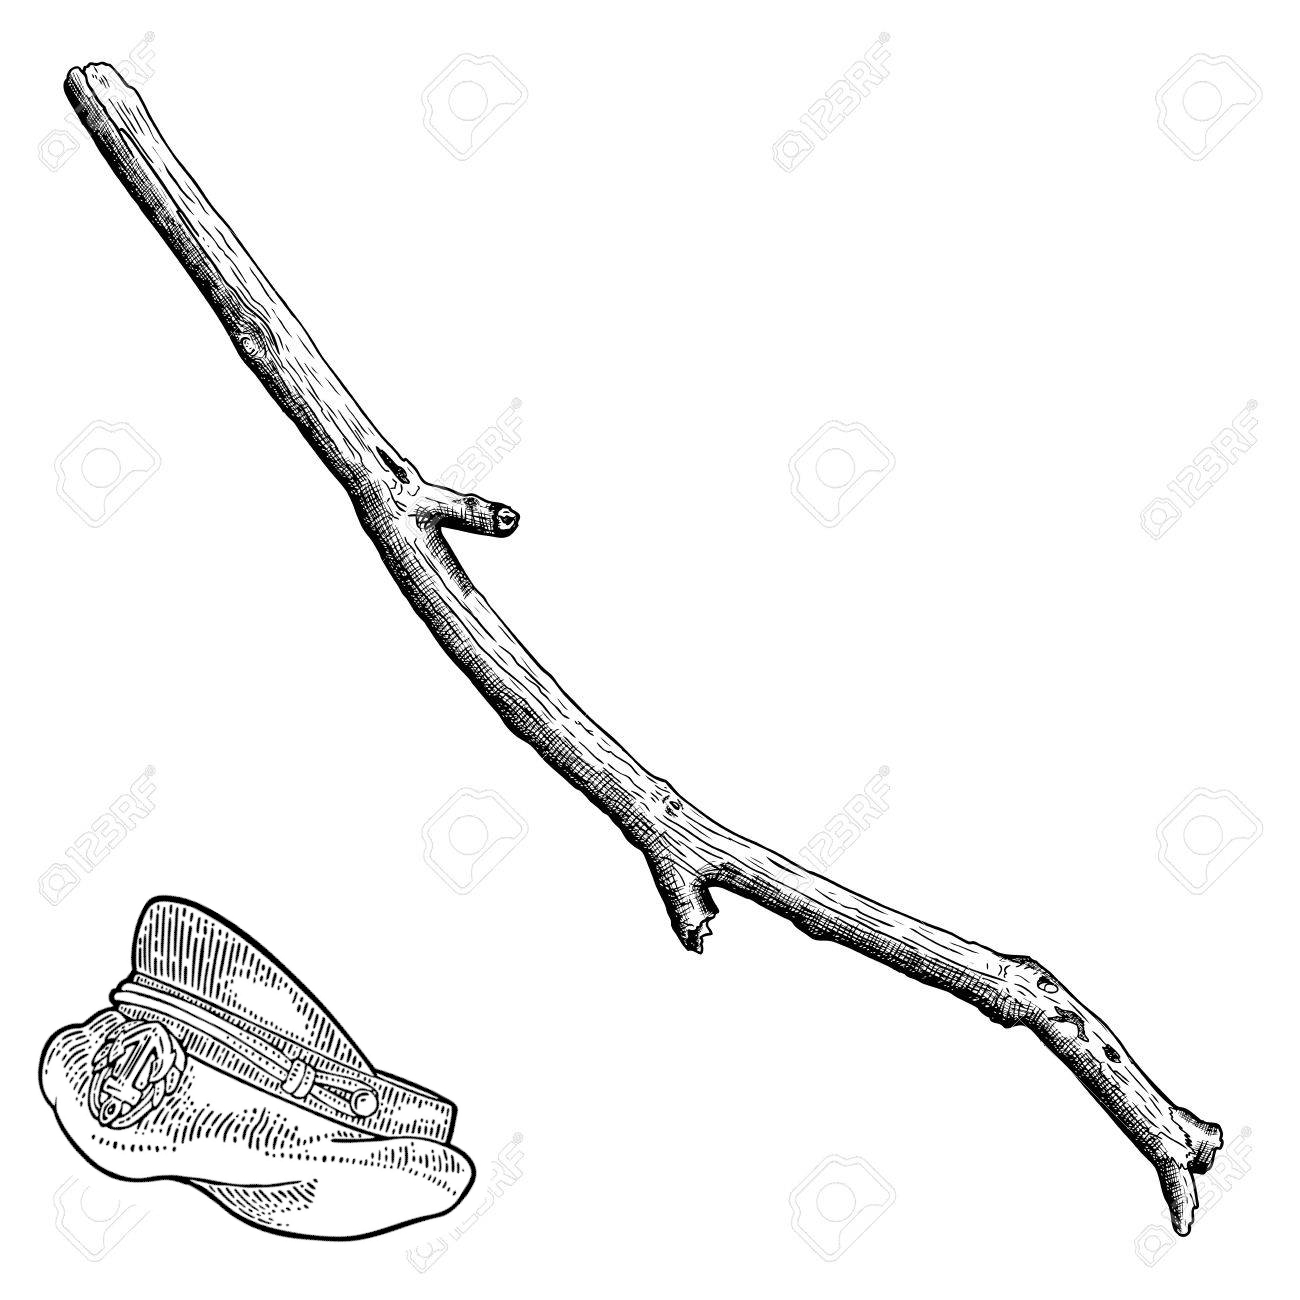
\includegraphics[width=\textwidth]{./content/img/xxx.jpg}
\begin{figure}[h]
\end{figure}
\end{center}

\clearpage
